% Options for packages loaded elsewhere
\PassOptionsToPackage{unicode}{hyperref}
\PassOptionsToPackage{hyphens}{url}
%
\documentclass[
  man,floatsintext]{apa6}
\usepackage{amsmath,amssymb}
\usepackage{iftex}
\ifPDFTeX
  \usepackage[T1]{fontenc}
  \usepackage[utf8]{inputenc}
  \usepackage{textcomp} % provide euro and other symbols
\else % if luatex or xetex
  \usepackage{unicode-math} % this also loads fontspec
  \defaultfontfeatures{Scale=MatchLowercase}
  \defaultfontfeatures[\rmfamily]{Ligatures=TeX,Scale=1}
\fi
\usepackage{lmodern}
\ifPDFTeX\else
  % xetex/luatex font selection
\fi
% Use upquote if available, for straight quotes in verbatim environments
\IfFileExists{upquote.sty}{\usepackage{upquote}}{}
\IfFileExists{microtype.sty}{% use microtype if available
  \usepackage[]{microtype}
  \UseMicrotypeSet[protrusion]{basicmath} % disable protrusion for tt fonts
}{}
\makeatletter
\@ifundefined{KOMAClassName}{% if non-KOMA class
  \IfFileExists{parskip.sty}{%
    \usepackage{parskip}
  }{% else
    \setlength{\parindent}{0pt}
    \setlength{\parskip}{6pt plus 2pt minus 1pt}}
}{% if KOMA class
  \KOMAoptions{parskip=half}}
\makeatother
\usepackage{xcolor}
\usepackage{color}
\usepackage{fancyvrb}
\newcommand{\VerbBar}{|}
\newcommand{\VERB}{\Verb[commandchars=\\\{\}]}
\DefineVerbatimEnvironment{Highlighting}{Verbatim}{commandchars=\\\{\}}
% Add ',fontsize=\small' for more characters per line
\usepackage{framed}
\definecolor{shadecolor}{RGB}{248,248,248}
\newenvironment{Shaded}{\begin{snugshade}}{\end{snugshade}}
\newcommand{\AlertTok}[1]{\textcolor[rgb]{0.94,0.16,0.16}{#1}}
\newcommand{\AnnotationTok}[1]{\textcolor[rgb]{0.56,0.35,0.01}{\textbf{\textit{#1}}}}
\newcommand{\AttributeTok}[1]{\textcolor[rgb]{0.13,0.29,0.53}{#1}}
\newcommand{\BaseNTok}[1]{\textcolor[rgb]{0.00,0.00,0.81}{#1}}
\newcommand{\BuiltInTok}[1]{#1}
\newcommand{\CharTok}[1]{\textcolor[rgb]{0.31,0.60,0.02}{#1}}
\newcommand{\CommentTok}[1]{\textcolor[rgb]{0.56,0.35,0.01}{\textit{#1}}}
\newcommand{\CommentVarTok}[1]{\textcolor[rgb]{0.56,0.35,0.01}{\textbf{\textit{#1}}}}
\newcommand{\ConstantTok}[1]{\textcolor[rgb]{0.56,0.35,0.01}{#1}}
\newcommand{\ControlFlowTok}[1]{\textcolor[rgb]{0.13,0.29,0.53}{\textbf{#1}}}
\newcommand{\DataTypeTok}[1]{\textcolor[rgb]{0.13,0.29,0.53}{#1}}
\newcommand{\DecValTok}[1]{\textcolor[rgb]{0.00,0.00,0.81}{#1}}
\newcommand{\DocumentationTok}[1]{\textcolor[rgb]{0.56,0.35,0.01}{\textbf{\textit{#1}}}}
\newcommand{\ErrorTok}[1]{\textcolor[rgb]{0.64,0.00,0.00}{\textbf{#1}}}
\newcommand{\ExtensionTok}[1]{#1}
\newcommand{\FloatTok}[1]{\textcolor[rgb]{0.00,0.00,0.81}{#1}}
\newcommand{\FunctionTok}[1]{\textcolor[rgb]{0.13,0.29,0.53}{\textbf{#1}}}
\newcommand{\ImportTok}[1]{#1}
\newcommand{\InformationTok}[1]{\textcolor[rgb]{0.56,0.35,0.01}{\textbf{\textit{#1}}}}
\newcommand{\KeywordTok}[1]{\textcolor[rgb]{0.13,0.29,0.53}{\textbf{#1}}}
\newcommand{\NormalTok}[1]{#1}
\newcommand{\OperatorTok}[1]{\textcolor[rgb]{0.81,0.36,0.00}{\textbf{#1}}}
\newcommand{\OtherTok}[1]{\textcolor[rgb]{0.56,0.35,0.01}{#1}}
\newcommand{\PreprocessorTok}[1]{\textcolor[rgb]{0.56,0.35,0.01}{\textit{#1}}}
\newcommand{\RegionMarkerTok}[1]{#1}
\newcommand{\SpecialCharTok}[1]{\textcolor[rgb]{0.81,0.36,0.00}{\textbf{#1}}}
\newcommand{\SpecialStringTok}[1]{\textcolor[rgb]{0.31,0.60,0.02}{#1}}
\newcommand{\StringTok}[1]{\textcolor[rgb]{0.31,0.60,0.02}{#1}}
\newcommand{\VariableTok}[1]{\textcolor[rgb]{0.00,0.00,0.00}{#1}}
\newcommand{\VerbatimStringTok}[1]{\textcolor[rgb]{0.31,0.60,0.02}{#1}}
\newcommand{\WarningTok}[1]{\textcolor[rgb]{0.56,0.35,0.01}{\textbf{\textit{#1}}}}
\usepackage{graphicx}
\makeatletter
\def\maxwidth{\ifdim\Gin@nat@width>\linewidth\linewidth\else\Gin@nat@width\fi}
\def\maxheight{\ifdim\Gin@nat@height>\textheight\textheight\else\Gin@nat@height\fi}
\makeatother
% Scale images if necessary, so that they will not overflow the page
% margins by default, and it is still possible to overwrite the defaults
% using explicit options in \includegraphics[width, height, ...]{}
\setkeys{Gin}{width=\maxwidth,height=\maxheight,keepaspectratio}
% Set default figure placement to htbp
\makeatletter
\def\fps@figure{htbp}
\makeatother
\setlength{\emergencystretch}{3em} % prevent overfull lines
\providecommand{\tightlist}{%
  \setlength{\itemsep}{0pt}\setlength{\parskip}{0pt}}
\setcounter{secnumdepth}{-\maxdimen} % remove section numbering
% Make \paragraph and \subparagraph free-standing
\ifx\paragraph\undefined\else
  \let\oldparagraph\paragraph
  \renewcommand{\paragraph}[1]{\oldparagraph{#1}\mbox{}}
\fi
\ifx\subparagraph\undefined\else
  \let\oldsubparagraph\subparagraph
  \renewcommand{\subparagraph}[1]{\oldsubparagraph{#1}\mbox{}}
\fi
% definitions for citeproc citations
\NewDocumentCommand\citeproctext{}{}
\NewDocumentCommand\citeproc{mm}{%
  \begingroup\def\citeproctext{#2}\cite{#1}\endgroup}
\makeatletter
 % allow citations to break across lines
 \let\@cite@ofmt\@firstofone
 % avoid brackets around text for \cite:
 \def\@biblabel#1{}
 \def\@cite#1#2{{#1\if@tempswa , #2\fi}}
\makeatother
\newlength{\cslhangindent}
\setlength{\cslhangindent}{1.5em}
\newlength{\csllabelwidth}
\setlength{\csllabelwidth}{3em}
\newenvironment{CSLReferences}[2] % #1 hanging-indent, #2 entry-spacing
 {\begin{list}{}{%
  \setlength{\itemindent}{0pt}
  \setlength{\leftmargin}{0pt}
  \setlength{\parsep}{0pt}
  % turn on hanging indent if param 1 is 1
  \ifodd #1
   \setlength{\leftmargin}{\cslhangindent}
   \setlength{\itemindent}{-1\cslhangindent}
  \fi
  % set entry spacing
  \setlength{\itemsep}{#2\baselineskip}}}
 {\end{list}}
\usepackage{calc}
\newcommand{\CSLBlock}[1]{\hfill\break#1\hfill\break}
\newcommand{\CSLLeftMargin}[1]{\parbox[t]{\csllabelwidth}{\strut#1\strut}}
\newcommand{\CSLRightInline}[1]{\parbox[t]{\linewidth - \csllabelwidth}{\strut#1\strut}}
\newcommand{\CSLIndent}[1]{\hspace{\cslhangindent}#1}
\ifLuaTeX
\usepackage[bidi=basic]{babel}
\else
\usepackage[bidi=default]{babel}
\fi
\babelprovide[main,import]{english}
% get rid of language-specific shorthands (see #6817):
\let\LanguageShortHands\languageshorthands
\def\languageshorthands#1{}
% Manuscript styling
\usepackage{upgreek}
\captionsetup{font=singlespacing,justification=justified}

% Table formatting
\usepackage{longtable}
\usepackage{lscape}
% \usepackage[counterclockwise]{rotating}   % Landscape page setup for large tables
\usepackage{multirow}		% Table styling
\usepackage{tabularx}		% Control Column width
\usepackage[flushleft]{threeparttable}	% Allows for three part tables with a specified notes section
\usepackage{threeparttablex}            % Lets threeparttable work with longtable

% Create new environments so endfloat can handle them
% \newenvironment{ltable}
%   {\begin{landscape}\centering\begin{threeparttable}}
%   {\end{threeparttable}\end{landscape}}
\newenvironment{lltable}{\begin{landscape}\centering\begin{ThreePartTable}}{\end{ThreePartTable}\end{landscape}}

% Enables adjusting longtable caption width to table width
% Solution found at http://golatex.de/longtable-mit-caption-so-breit-wie-die-tabelle-t15767.html
\makeatletter
\newcommand\LastLTentrywidth{1em}
\newlength\longtablewidth
\setlength{\longtablewidth}{1in}
\newcommand{\getlongtablewidth}{\begingroup \ifcsname LT@\roman{LT@tables}\endcsname \global\longtablewidth=0pt \renewcommand{\LT@entry}[2]{\global\advance\longtablewidth by ##2\relax\gdef\LastLTentrywidth{##2}}\@nameuse{LT@\roman{LT@tables}} \fi \endgroup}

% \setlength{\parindent}{0.5in}
% \setlength{\parskip}{0pt plus 0pt minus 0pt}

% Overwrite redefinition of paragraph and subparagraph by the default LaTeX template
% See https://github.com/crsh/papaja/issues/292
\makeatletter
\renewcommand{\paragraph}{\@startsection{paragraph}{4}{\parindent}%
  {0\baselineskip \@plus 0.2ex \@minus 0.2ex}%
  {-1em}%
  {\normalfont\normalsize\bfseries\itshape\typesectitle}}

\renewcommand{\subparagraph}[1]{\@startsection{subparagraph}{5}{1em}%
  {0\baselineskip \@plus 0.2ex \@minus 0.2ex}%
  {-\z@\relax}%
  {\normalfont\normalsize\itshape\hspace{\parindent}{#1}\textit{\addperi}}{\relax}}
\makeatother

% \usepackage{etoolbox}
\makeatletter
\patchcmd{\HyOrg@maketitle}
  {\section{\normalfont\normalsize\abstractname}}
  {\section*{\normalfont\normalsize\abstractname}}
  {}{\typeout{Failed to patch abstract.}}
\patchcmd{\HyOrg@maketitle}
  {\section{\protect\normalfont{\@title}}}
  {\section*{\protect\normalfont{\@title}}}
  {}{\typeout{Failed to patch title.}}
\makeatother

\usepackage{xpatch}
\makeatletter
\xapptocmd\appendix
  {\xapptocmd\section
    {\addcontentsline{toc}{section}{\appendixname\ifoneappendix\else~\theappendix\fi\\: #1}}
    {}{\InnerPatchFailed}%
  }
{}{\PatchFailed}
\keywords{ordinal, likert, simulations, power\newline\indent Word count: X}
\usepackage{csquotes}
\ifLuaTeX
  \usepackage{selnolig}  % disable illegal ligatures
\fi
\IfFileExists{bookmark.sty}{\usepackage{bookmark}}{\usepackage{hyperref}}
\IfFileExists{xurl.sty}{\usepackage{xurl}}{} % add URL line breaks if available
\urlstyle{same}
\hypersetup{
  pdftitle={Ordinal regression models made easy. A tutorial on parameter interpretation, data simulation, and power analysis.},
  pdfauthor={Filippo Gambarota1 \& Gianmarco Altoè1},
  pdflang={en-EN},
  pdfkeywords={ordinal, likert, simulations, power},
  hidelinks,
  pdfcreator={LaTeX via pandoc}}

\title{Ordinal regression models made easy. A tutorial on parameter interpretation, data simulation, and power analysis.}
\author{Filippo Gambarota\textsuperscript{1} \& Gianmarco Altoè\textsuperscript{1}}
\date{}


\shorttitle{Ordinal regression models made easy}

\authornote{

Add complete departmental affiliations for each author here. Each new line herein must be indented, like this line.

Enter author note here.

The authors made the following contributions. Filippo Gambarota: Conceptualization, Writing - Original Draft Preparation, Writing - Review \& Editing; Gianmarco Altoè: Writing - Review \& Editing, Supervision.

Correspondence concerning this article should be addressed to Filippo Gambarota, Postal address. E-mail: \href{mailto:filippo.gambarota@unipd.it}{\nolinkurl{filippo.gambarota@unipd.it}}

}

\affiliation{\vspace{0.5cm}\textsuperscript{1} Department of Developmental Psychology and Socialization, University of Padova, Italy}

\abstract{%
Abstract here
}



\begin{document}
\maketitle

\section{Introduction}\label{introduction}

Psychological research make an extensive use of ordinal data. One of the main reason is probably the usage of Likert scales (Likert, 1932). Ordinal data refers to a specific type of measurement scale (Stevens, 1946) where ordered numbers are assigned to a variable. Compared to nominal scale and as the name suggest the labels are ordered. Compared to interval or ratio scales there is no explicit assumption about the distance between labels. (rivedi questo). An example is asking people the degree of agreement about a certain statement using a scale from 1 (no agreement) to 7 (total agreement). Answering 4 compared to 2 suggest an higher agreement but we cannot affirm that there is two times the agreement compared to the second answer. Stevens (1946) and Kemp and Grace (2021) suggested that for ordinal variables is appropriate to calculate ranks-based statistics (e.g., median or percentiles) instead of metric statistics (e.g., mean or standard deviation). This distinction in terms of the appropriateness of certain descriptive statistics is also relevant when modeling data. Treating ordinal data as metric refers to assuming the labels as actual integer numbers thus assuming a fixed and know distance between levels (Liddell \& Kruschke, 2018).

In Psychology especially when using item-based measures (questionnaires, surveys, etc.) the common practice is using a normal linear regression that makes an explicit assumption about metric features of the response variable. Liddell and Kruschke (2018) reviewed the psychological literature using likert-based measures and reported how the majority of papers used metric-based statistical models. In the same work, Liddell and Kruschke (2018) showed extensive examples and simulations about the potential pitfalls of treating an ordinal variable as metric (but see Robitzsch, 2020 for an alternative perspective). They reported problems in terms of lack of power, inversion of the effects and distortion in estimating the effect size (rivedi meglio qui). (vedi se c'è qualche altro lavoro che fa vedere questa cosa). Some authors suggested that despite individual items being ordinal, averaging multiple items could solve the problem of applying metric models (e.g., Carifio \& Perla, 2007, 2008 metti queste citazioni). Liddell and Kruschke (2018) suggested that in some conditions even averaging multiple items and applying metric models could be problematic. Cliff (2016) suggest that most of the research questions in behavioral sciences can be considered as ordinal (\emph{is the score \(x\) higher than the score \(y\)}?) concerning variables where the most appropriate measurement scale is probably ordinal.

qualcosa ancora qui

\subsection{Ordinal regression models}\label{ordinal-regression-models}

Despite the actual modeling proposal by Liddell and Kruschke (2018), there is a class of regression models taking into account the ordinal nature of the response variable without making metric assumptions. We can class this general class of models as \emph{ordinal regression}. The nomenclature of these models can be confusing mainly because there are several subclasses of models with different assumptions and structures (Gerhard Tutz, 2022). Gerhard Tutz (2022) and Bürkner and Vuorre (2019) provide a clear and updated taxonomy of ordinal regression models. We can identify three main classes: \emph{cumulative models} (McCullagh, 1980), \emph{sequential models} (Gerhard Tutz, 1990) and \emph{adjacent category models}. The cumulative is the mostly used model assuming the existence of a latent variable that when segmented using thresholds produces the observed ordinal variable. The psychological process underlying the response is clearly formalized in the signal detection theory framework where the respondent (vedi come sistemare). The sequential model as suggested by the name is appropriate when modelling sequential processes. Assuming to have 5 response options, the sequential model assume that responding 3 means already reaching the states 1 and 2. A clear example is proposed by Bürkner and Vuorre (2019) where the marriage duration in years is predicted as a function of some explanatory variables. For each level of the response variable there is a latent distribution where the step between a marriage year \(k = 1\) and the next years \(k > 1\) is modeled by the sequential regression. When comparing \(k\) with \(k > 1\), everything lower than \(k\) is assumed to be already reached (Gerhard Tutz \& Berger, 2020). The adjacent category model compare the category \(k\) with \(k + 1\) still assuming a latent distribution for each \(k\). As suggested by Gerhard Tutz (2022) the adjacent-category model can be seen as a series of binary binomial regressions taking into account the order of the categories. Bürkner and Vuorre (2019) suggested that adjacent-category model can be chosen for its mathematical convenience and there is no a clear empirical distinction as for the cumulative vs sequential model.

In the current paper we put the focus on the cumulative model for several reasons. The first reason is that the latent formulation of the model is particularly convenient both for parameter interpretation and data simulation. The second reason is that several psychological variables can be formalized as a latent continuous construct that when measured is collected using ordinal items. Furthermore, also the signal detection theory framework models the decision process assuming a latent distribution for the signal and noise where thresholds are the response criteria (e.g., DeCarlo, 2010).

\scriptsize

\begin{figure}

{\centering \includegraphics[width=1\linewidth]{img/fig-ordinal-models} 

}

\caption{Theoretical figure about ordinal models. Voglio fare una figura come questa in Bürkner and Vuorre (2019) ma con qualche modifica per fare vedere i tre modelli.}\label{fig:fig-ordinal-models}
\end{figure}

\normalsize

\subsection{Model notation}\label{model-notation}

metti qualcosa sulla nomenclatura

\begin{quote}
The name, cumulative link models is adopted from Agresti (2002), but the model class has
been referred to by several other names in the literature, such as ordered logit models and
ordered probit models (Greene and Hensher 2010) for the logit and probit link functions. The
cumulative link model with a logit link is widely known as the proportional odds model due
to McCullagh (1980) and with a complementary log-log link, the model is sometimes referred
to as the proportional hazards model for grouped survival times.
\end{quote}

In this section we introduce some notations for the cumulative model that is used through the paper and in the R code. The notation is as consistent as possible with the main textbooks and with the \texttt{ordinal} R package used in the tutorial. We define \(Y_k\) as the observed ordinal response with \(1, 2, \dots,k\) options and \(Y^\star\) is the corresponding latent variable. The latent variable is segmented using \(k - 1\) thresholds \(\alpha_1, \alpha_2, \dots, \alpha_{k - 1}\). With \(g()\) we define the cumulative probability function assumed for the specific model. For example, when using a Gaussian distribution we are fitting a model with a \texttt{probit} link function thus \(f() = \Phi()\). With \(g^{-1}()\) we define the inverse of the cumulative probability function. The minus sign in \(\mathbf{X}\mathbf{\beta}\) is used to give the usual interpretation of standard regression models where an increase in \(\beta\) corresponds to an increase in the probability of higher categories of \(Y\) (metti il libro di agresti sui dati ordinali).

\begin{equation} 
P(Y \leq k) = g(\alpha_k - \mathbf{X} \mathbf{\beta}), \;\;k = 1, 2, \dots, k
\label{eq:prob-cum-model1}
\end{equation}

We can call the \(\mathbf{X}\mathbf{\beta}\) as the linear predictor \(\eta\). Equation (num) describe how the probability of a single outcome \(Y_k\).

\begin{equation} 
P(Y = k) = g^{-1}(\alpha_k - \eta) -  g^{-1}(\alpha_{k - 1} - \eta)
\label{eq:prob-cum-model2}
\end{equation}

The same model can be formalized using the latent formulation (see Equation). This is more similar to a standard linear regression.

\begin{equation} 
Y^\star_i = \eta + \epsilon_i
\label{eq:latent-model}
\end{equation}

Where \(\epsilon\) is the error part and comes from the distribution that is assumed from the latent model. For a \emph{probit} model, errors are sampled from a standard Gaussian distribution while for a \emph{logit} model from a standard logistic distribution. Then the observed ordinal value \(Y_i\) comes from \(Y^\star_i\) being between the thresholds \(\alpha_{k - 1} < Y^\star_i < \alpha_{k}\) with thresholds organized as \(- \infty \equiv \alpha_1 < \dots< \alpha_{k - 1} < \alpha_k \equiv \infty\).

In the basic version of the model, the thresholds \(\alpha\) are considered as fixed and do not vary as a function of predictors. The thresholds are part of the measurement procedure (Liddell \& Kruschke, 2018). In a more sophisticated version of the model called location-shift (Gerhard Tutz, 2022), both the location \(\mu\) and the thresholds \(\alpha\) can vary as a function of the predictors. In the following sections another version of the model called location-scale (Cox, 1995; Rigby \& Stasinopoulos, 2005; Gerhard Tutz, 2022) will be presented as a more flexible way to model latent distributions with heterogeneous variance (spiega meglio).

\subsection{lm on latent vs ordinal}\label{lm-on-latent-vs-ordinal}

as suggested \url{https://people.vcu.edu/~dbandyop/BIOS625/CLM_R.pdf}, running a lm on the latent variables gives similar parameter as the clm. Of course, we are able to do this with real data given that the ordinal variable is the observed version of an unobserved latent variable. But in simulation this is useful to understand what the cumulative model is doing.

\scriptsize

\begin{verbatim}
## 
## Call:
## lm(formula = ys ~ x1 + x2, data = dat)
## 
## Residuals:
##     Min      1Q  Median      3Q     Max 
## -4.4772 -0.6765 -0.0005  0.6742  4.0796 
## 
## Coefficients:
##              Estimate Std. Error t value Pr(>|t|)    
## (Intercept) 0.0007926  0.0031780   0.249    0.803    
## x1          1.0009911  0.0031859 314.192   <2e-16 ***
## x2          0.4998991  0.0031800 157.203   <2e-16 ***
## ---
## Signif. codes:  0 '***' 0.001 '**' 0.01 '*' 0.05 '.' 0.1 ' ' 1
## 
## Residual standard error: 1.005 on 99997 degrees of freedom
## Multiple R-squared:  0.5514, Adjusted R-squared:  0.5513 
## F-statistic: 6.144e+04 on 2 and 99997 DF,  p-value: < 2.2e-16
\end{verbatim}

\begin{verbatim}
## formula: y ~ x1 + x2
## data:    dat
## 
##  link   threshold nobs  logLik     AIC       niter max.grad cond.H 
##  probit flexible  1e+05 -122909.88 245831.76 5(0)  2.04e-07 9.1e+00
## 
## Coefficients:
##     x1     x2 
## 0.9949 0.4965 
## 
## Threshold coefficients:
##     1|2     2|3     3|4     4|5 
## -0.8360 -0.2568  0.2515  0.8421
\end{verbatim}

\begin{verbatim}
##  (Intercept)           x1           x2 
## 0.0007886378 0.9960398259 0.4974264662
\end{verbatim}

\normalsize

\subsection{Kruscke parametrization}\label{kruscke-parametrization}

Liddell and Kruschke (2018) and Kruschke (2015) proposed an alternative parametrization to understand the model parameters. They used a probit model where thresholds and regression parameters are estimated on the scale of the ordinal variable compared to standard ordinal regression where they refers to the quantile of the latent variables for the threshold and z score or odds ratio for the regression coefficients. They implemented the model in Jags and provided some equations and R functions to convert from the standard parametrization to the proposed one.

The proposed model is fitted within a Bayesian framework using either Jags (citation) or Stan (citation). Kruskche proposed a simple method to convert the parameters fitted with a standard model within the proposed parametriazion. The main improvement regards mapping the values (for thresholds \(\alpha_i\) and slopes \(\beta\)) from latent standard distribution (gaussian or logistic) into the scale of the \(y\) ordinal value. The scale of the variable depend on the numeric labels assigned to ordered categories. There is an additional feature of the proposed parametrization where the first and the last thresholds are fixed respectively to \(\alpha_1 + 0.5\) and \(\alpha_k - 0.5\) where other thresholds are estimated.

Kurz (2023) explain how to convert a model fitted with the \texttt{brms} package (citation) (an R package for regression modeling using \emph{stan}) into the Kruschke (2015) parametrization.

Using the function proposed by Kruschke (2015) (metti ref ad osf) and the equations presented in Kurz (2023) the \texttt{clm\_to\_ord()} function convert parameters fitted with the \texttt{clm} function into the corresponding parameters for the latent \(Y^\star\) variable considering the actual range of values (from 1 to \(k\)).

\scriptsize

\begin{Shaded}
\begin{Highlighting}[]
\NormalTok{clm\_to\_ord }\OtherTok{\textless{}{-}} \ControlFlowTok{function}\NormalTok{(fit)\{}
\NormalTok{  th }\OtherTok{\textless{}{-}} \FunctionTok{unname}\NormalTok{(fit}\SpecialCharTok{$}\NormalTok{alpha) }\CommentTok{\# estimated thresholds}
\NormalTok{  coefs }\OtherTok{\textless{}{-}}\NormalTok{ fit}\SpecialCharTok{$}\NormalTok{coefficients}
\NormalTok{  coefs }\OtherTok{\textless{}{-}} \FunctionTok{unname}\NormalTok{(coefs[(}\FunctionTok{length}\NormalTok{(th) }\SpecialCharTok{+} \DecValTok{1}\NormalTok{)}\SpecialCharTok{:}\FunctionTok{length}\NormalTok{(coefs)])}
\NormalTok{  k }\OtherTok{\textless{}{-}} \FunctionTok{length}\NormalTok{(th) }\SpecialCharTok{+} \DecValTok{1} \CommentTok{\# number of levels for y}
\NormalTok{  y }\OtherTok{\textless{}{-}} \DecValTok{1}\SpecialCharTok{:}\NormalTok{k }\CommentTok{\# ordinal values}
\NormalTok{  stdm }\OtherTok{\textless{}{-}} \DecValTok{0} \CommentTok{\# latent mean}
\NormalTok{  stds }\OtherTok{\textless{}{-}} \DecValTok{1} \CommentTok{\# latent sigma}
\NormalTok{  th\_y }\OtherTok{\textless{}{-}}\NormalTok{ scales}\SpecialCharTok{::}\FunctionTok{rescale}\NormalTok{(th, }\AttributeTok{to =} \FunctionTok{c}\NormalTok{(y[}\DecValTok{1}\NormalTok{] }\SpecialCharTok{+} \FloatTok{0.5}\NormalTok{, y[k] }\SpecialCharTok{{-}} \FloatTok{0.5}\NormalTok{))}
\NormalTok{  lats }\OtherTok{\textless{}{-}}\NormalTok{ (th\_y[}\DecValTok{2}\NormalTok{] }\SpecialCharTok{{-}}\NormalTok{ th\_y[k }\SpecialCharTok{{-}} \DecValTok{2}\NormalTok{]) }\SpecialCharTok{/}\NormalTok{ (th[}\DecValTok{2}\NormalTok{] }\SpecialCharTok{{-}}\NormalTok{ th[k }\SpecialCharTok{{-}} \DecValTok{2}\NormalTok{]) }\CommentTok{\# real latent sigma}
\NormalTok{  b0 }\OtherTok{\textless{}{-}}\NormalTok{ th\_y[}\DecValTok{1}\NormalTok{] }\SpecialCharTok{{-}}\NormalTok{ th[}\DecValTok{1}\NormalTok{] }\SpecialCharTok{*}\NormalTok{ lats}
\NormalTok{  betas }\OtherTok{\textless{}{-}}\NormalTok{ lats }\SpecialCharTok{*}\NormalTok{ coefs}
\NormalTok{  out }\OtherTok{\textless{}{-}} \FunctionTok{list}\NormalTok{(}\AttributeTok{sigma =}\NormalTok{ lats, }\AttributeTok{b0 =}\NormalTok{ b0, }\AttributeTok{beta =}\NormalTok{ betas, }\AttributeTok{alpha =}\NormalTok{ th\_y)}
  \FunctionTok{return}\NormalTok{(out)}
\NormalTok{\}}
\end{Highlighting}
\end{Shaded}

\normalsize

\scriptsize

\begin{Shaded}
\begin{Highlighting}[]
\NormalTok{dat }\OtherTok{\textless{}{-}} \FunctionTok{data.frame}\NormalTok{(}
  \AttributeTok{x =} \FunctionTok{rnorm}\NormalTok{(}\FloatTok{1e5}\NormalTok{)}
\NormalTok{)}

\NormalTok{dat }\OtherTok{\textless{}{-}} \FunctionTok{sim\_ord\_latent}\NormalTok{(}\SpecialCharTok{\textasciitilde{}}\NormalTok{x, }\AttributeTok{By =} \DecValTok{1}\NormalTok{, }\AttributeTok{probs =} \FunctionTok{rep}\NormalTok{(}\DecValTok{1}\SpecialCharTok{/}\DecValTok{5}\NormalTok{, }\DecValTok{5}\NormalTok{), }\AttributeTok{link =} \StringTok{"probit"}\NormalTok{, }\AttributeTok{data =}\NormalTok{ dat)}
\NormalTok{fit }\OtherTok{\textless{}{-}} \FunctionTok{clm}\NormalTok{(y }\SpecialCharTok{\textasciitilde{}}\NormalTok{ x, }\AttributeTok{data =}\NormalTok{ dat, }\AttributeTok{link =} \StringTok{"probit"}\NormalTok{)}
\FunctionTok{clm\_to\_ord}\NormalTok{(fit)}
\end{Highlighting}
\end{Shaded}

\begin{verbatim}
## $sigma
## [1] 1.78472
## 
## $b0
## [1] 2.993037
## 
## $beta
## [1] 1.797978
## 
## $alpha
## [1] 1.500000 2.560652 3.446266 4.500000
\end{verbatim}

\normalsize

\subsection{Gelman parametrization}\label{gelman-parametrization}

rivedi questa parametrizzazione in Gelman, Hill, and Vehtari (2020)

\scriptsize

\normalsize

\section{Interpreting parameters}\label{interpreting-parameters}

\subsection{Odds and odds ratio}\label{odds-and-odds-ratio}

una piccola spiegazione di odds e odds ratio

\subsection{Proportional odds assumption}\label{proportional-odds-assumption}

Following again the taxonomy by Gerhard Tutz (2022), each of the presented ordinal regression model has a basic version making the proportional odds assumption. There are more advanced versions of the model relaxing this assumption completely (\emph{non proportional odds} models) and partially (\emph{partial proportional odds} models) (rivedi se la nomenclatura va bene). The proportional odds assumption is a crucial point when intepreting model parameters. Can be formalized as in Equation (). Basically if we use the \emph{logit} link function \(g()\) the \(\beta\)s are interpreted as standard odds ratio in the logistic regression. Given that we have \(k > 2\) alternatives there is the need of \(k - 1\) equations (as reported in Equation ()). The porportional odds is assuming that the regression coefficients \(\beta\) are independent from the thresholds \(\alpha\) thus the effect is the same regardless of the \(Y\) level. Thus \(\beta_1 = \beta_2 \dots = \beta_{k - 1}\). The Figure () depicts the proportional odds assumption for the \(k - 1\) logistic curves both for probabilities and linear predictors \(\eta\).

\scriptsize

\begin{figure}

{\centering \includegraphics{paper-new_files/figure-latex/fig-prop-odds-1} 

}

\caption{caption here}\label{fig:fig-prop-odds}
\end{figure}

\normalsize

The proportional odds assumption is convenient because regardless the number of \(k\), the \(\beta_j\) (\(j\) being the number of regression coefficients) effect is assumed to be the same. The model is more parsimonious compared to estimating \(k - 1\) coefficients for each \(\beta_j\) as in the multinomial regression or the non-proportional version of the ordinal regression. Clearly this can be a strong assumption in some conditions. There are several methods to test the proportional odds assumption (see Liu, He, Tu, \& Tang, 2023 for an overview). Gerhard Tutz and Berger (2020) suggested that using alternative as the location-shift or location-scale models, the assumption can be made (improving model parsimony) but still having a more flexible modeling framework. In the next section, we provide more details about the location-scale model in terms of parameters interpretation and data simulation.

\subsection{Demonstrating the proportional odds assumption}\label{demonstrating-the-proportional-odds-assumption}

basically given that the effect of \(\beta\) is constant the odds ratio is independent from the thresholds \(\alpha_j\) (Liu et al., 2023). In the current paper we are simulating data using a single set of \(\beta\)s thus the proportional odds assumption is true. Liu et al. (2023) reviewed the available methods to test this assumption.

\begin{itemize}
\tightlist
\item
  \url{https://hbiostat.org/ordinal/impactpo.pdf} blog su proportional odds, mi pare di capire che non sia così problematica come assunzione
\end{itemize}

sarebbe da capire quali sono i rischi di assumere questo ed eventualmente se simulare non proportional odds è troppo complicato.

Let's simulate the effect of a binary predictor on ordinal scale 1-5:

\scriptsize

\begin{Shaded}
\begin{Highlighting}[]
\NormalTok{b1 }\OtherTok{\textless{}{-}} \FunctionTok{log}\NormalTok{(}\DecValTok{3}\NormalTok{) }\CommentTok{\# log odds ratio}
\NormalTok{n }\OtherTok{\textless{}{-}} \FloatTok{1e4}
\NormalTok{x }\OtherTok{\textless{}{-}} \FunctionTok{rep}\NormalTok{(}\FunctionTok{c}\NormalTok{(}\StringTok{"a"}\NormalTok{, }\StringTok{"b"}\NormalTok{), }\AttributeTok{each =}\NormalTok{ n}\SpecialCharTok{/}\DecValTok{2}\NormalTok{)}
\NormalTok{dat }\OtherTok{\textless{}{-}} \FunctionTok{data.frame}\NormalTok{(}\AttributeTok{x =}\NormalTok{ x)}
\NormalTok{probs }\OtherTok{\textless{}{-}} \FunctionTok{rep}\NormalTok{(}\DecValTok{1}\SpecialCharTok{/}\DecValTok{5}\NormalTok{, }\DecValTok{5}\NormalTok{) }\CommentTok{\# for the group "a", uniform probabilities}
\NormalTok{dat }\OtherTok{\textless{}{-}} \FunctionTok{sim\_ord\_latent}\NormalTok{(}\SpecialCharTok{\textasciitilde{}}\NormalTok{x, }\AttributeTok{By =}\NormalTok{ b1, }\AttributeTok{probs =}\NormalTok{ probs, }\AttributeTok{data =}\NormalTok{ dat, }\AttributeTok{link =} \StringTok{"logit"}\NormalTok{)}
\NormalTok{fit }\OtherTok{\textless{}{-}} \FunctionTok{clm}\NormalTok{(y }\SpecialCharTok{\textasciitilde{}}\NormalTok{ x, }\AttributeTok{data =}\NormalTok{ dat, }\AttributeTok{link =} \StringTok{"logit"}\NormalTok{)}
\NormalTok{pr }\OtherTok{\textless{}{-}} \FunctionTok{predict}\NormalTok{(fit, }\FunctionTok{data.frame}\NormalTok{(}\AttributeTok{x =} \FunctionTok{unique}\NormalTok{(x)))}\SpecialCharTok{$}\NormalTok{fit}
\NormalTok{pr}
\end{Highlighting}
\end{Shaded}

\begin{verbatim}
##            1         2         3         4         5
## 1 0.20141151 0.2052163 0.2038036 0.1939345 0.1956341
## 2 0.07031792 0.1001600 0.1492126 0.2324907 0.4478188
\end{verbatim}

\normalsize
Basically the proportional odds suggest that:

\[
\text log(\frac{P(y \leq 1)}{P(y > 1)})
\]

Is the same regardless the level of the \(x\) predictor. Thus:

\[
\text{log}\left(\frac{\frac{P(y \leq 1|x_0)}{P(y > 1|x_0)}}{\frac{P(y \leq 2|x_0)}{P(y > 2|x_0)}}\right) = \text{log}\left(\frac{\frac{P(y \leq 1|x_1)}{P(y > 1|x_1)}}{\frac{P(y \leq 2|x_1)}{P(y > 2|x_1)}}\right)
\]

\scriptsize

\begin{Shaded}
\begin{Highlighting}[]
\NormalTok{a\_or1vs2345 }\OtherTok{\textless{}{-}}\NormalTok{ filor}\SpecialCharTok{::}\FunctionTok{odds}\NormalTok{(pr[}\DecValTok{1}\NormalTok{, }\DecValTok{1}\NormalTok{]) }\CommentTok{\# 1 vs 2 3 4 5}
\NormalTok{a\_or12vs345 }\OtherTok{\textless{}{-}}\NormalTok{ filor}\SpecialCharTok{::}\FunctionTok{odds}\NormalTok{(}\FunctionTok{sum}\NormalTok{(pr[}\DecValTok{1}\NormalTok{, }\DecValTok{1}\SpecialCharTok{:}\DecValTok{2}\NormalTok{])) }\CommentTok{\# 1 vs 2 3 4 5}

\NormalTok{b\_or1vs2345 }\OtherTok{\textless{}{-}}\NormalTok{ filor}\SpecialCharTok{::}\FunctionTok{odds}\NormalTok{(pr[}\DecValTok{2}\NormalTok{, }\DecValTok{1}\NormalTok{]) }\CommentTok{\# 1 vs 2 3 4 5}
\NormalTok{b\_or12vs345 }\OtherTok{\textless{}{-}}\NormalTok{ filor}\SpecialCharTok{::}\FunctionTok{odds}\NormalTok{(}\FunctionTok{sum}\NormalTok{(pr[}\DecValTok{2}\NormalTok{, }\DecValTok{1}\SpecialCharTok{:}\DecValTok{2}\NormalTok{])) }\CommentTok{\# 1 vs 2 3 4 5}

\FunctionTok{c}\NormalTok{(}\AttributeTok{xa =} \FunctionTok{log}\NormalTok{(a\_or1vs2345 }\SpecialCharTok{/}\NormalTok{ a\_or12vs345), }\AttributeTok{xb =} \FunctionTok{log}\NormalTok{(b\_or1vs2345 }\SpecialCharTok{/}\NormalTok{ b\_or12vs345))}
\end{Highlighting}
\end{Shaded}

\begin{verbatim}
##         xa         xb 
## -0.9995719 -0.9995719
\end{verbatim}

\normalsize

Proportional odds can be also visualized by plotting the cumulative probabilities of \(y\), in terms of \(g(P(y \leq j))\) (where \(g()\) is the logit link function) as a function of the predictor \(x\). If the proportional odds assumptions holds the slopes are parallel (also known as parallel regression assumption). The Figure \ref{fig:poa-plot-example} depicts the assumption of proportional odds in the probability and logit space.

\scriptsize

\begin{figure}

{\centering \includegraphics{paper-new_files/figure-latex/poa-plot-example-1} 

}

\caption{POA assumption}\label{fig:poa-plot-example}
\end{figure}

\normalsize

Harrell (2015) proposed a very intuitive plot to assess the proportional odds assumption and eventually the degree of deviation from the ideal case. Basically predictor is plotted against the logit of the cumulative probability. Distances between pairs of symbols should be similar across levels of the predictors. Numerical predictors can be binned before plotting the corresponding logit. Figure \ref{fig:harrel-poa-plot} depicts an example with simulated data satisfying the proportional odds assumption.

\scriptsize

\begin{figure}

{\centering \includegraphics{paper-new_files/figure-latex/harrel-poa-plot-1} 

}

\caption{Harrel Poa Plot}\label{fig:harrel-poa-plot}
\end{figure}

\normalsize

From a statistical point of view, the proportional odds assumption can be assessed by fitting \(k - 1\) binomial regressions and checking if the estimated \(\beta\) is similar between regressions. The regressions are estimated by creating \(k - 1\) dummy variables from the ordinal \(y\). The code below show that simulating data with the proportional odds create \(k - 1\) binomial regression with similar \(\beta\)s. In fact, fitting \(k - 1\) binomial regressions can be considered also an alternative to fitting an ordinal regression (see Gelman et al., 2020) with more flexibility in parameters (there will be \(k - 1\) regression coefficients instead of a single one) but losing the latent intepretation (magari qualcosa di più qui).

\scriptsize

\begin{Shaded}
\begin{Highlighting}[]
\NormalTok{k }\OtherTok{\textless{}{-}} \DecValTok{4}
\NormalTok{n }\OtherTok{\textless{}{-}} \FloatTok{1e5}
\NormalTok{dat }\OtherTok{\textless{}{-}} \FunctionTok{data.frame}\NormalTok{(}
  \AttributeTok{x =} \FunctionTok{runif}\NormalTok{(n)}
\NormalTok{)}

\NormalTok{dat }\OtherTok{\textless{}{-}} \FunctionTok{sim\_ord\_latent}\NormalTok{(}\SpecialCharTok{\textasciitilde{}}\NormalTok{x, }\AttributeTok{By =} \DecValTok{5}\NormalTok{, }\AttributeTok{probs =} \FunctionTok{rep}\NormalTok{(}\DecValTok{1}\SpecialCharTok{/}\NormalTok{k, k), }\AttributeTok{data =}\NormalTok{ dat, }\AttributeTok{link =} \StringTok{"logit"}\NormalTok{)}

\CommentTok{\# create dummy variables}

\NormalTok{dat}\SpecialCharTok{$}\NormalTok{y1vs234 }\OtherTok{\textless{}{-}} \FunctionTok{ifelse}\NormalTok{(dat}\SpecialCharTok{$}\NormalTok{y }\SpecialCharTok{\textless{}=} \DecValTok{1}\NormalTok{, }\DecValTok{1}\NormalTok{, }\DecValTok{0}\NormalTok{)}
\NormalTok{dat}\SpecialCharTok{$}\NormalTok{y12vs34 }\OtherTok{\textless{}{-}} \FunctionTok{ifelse}\NormalTok{(dat}\SpecialCharTok{$}\NormalTok{y }\SpecialCharTok{\textless{}=} \DecValTok{2}\NormalTok{, }\DecValTok{1}\NormalTok{, }\DecValTok{0}\NormalTok{)}
\NormalTok{dat}\SpecialCharTok{$}\NormalTok{y123vs4 }\OtherTok{\textless{}{-}} \FunctionTok{ifelse}\NormalTok{(dat}\SpecialCharTok{$}\NormalTok{y }\SpecialCharTok{\textless{}=} \DecValTok{3}\NormalTok{, }\DecValTok{1}\NormalTok{, }\DecValTok{0}\NormalTok{)}

\NormalTok{fit1vs234 }\OtherTok{\textless{}{-}} \FunctionTok{glm}\NormalTok{(y1vs234 }\SpecialCharTok{\textasciitilde{}}\NormalTok{ x, }\AttributeTok{data =}\NormalTok{ dat, }\AttributeTok{family =} \FunctionTok{binomial}\NormalTok{(}\AttributeTok{link =} \StringTok{"logit"}\NormalTok{))}
\NormalTok{fit12vs34 }\OtherTok{\textless{}{-}} \FunctionTok{glm}\NormalTok{(y12vs34 }\SpecialCharTok{\textasciitilde{}}\NormalTok{ x, }\AttributeTok{data =}\NormalTok{ dat, }\AttributeTok{family =} \FunctionTok{binomial}\NormalTok{(}\AttributeTok{link =} \StringTok{"logit"}\NormalTok{))}
\NormalTok{fit123vs4 }\OtherTok{\textless{}{-}} \FunctionTok{glm}\NormalTok{(y123vs4 }\SpecialCharTok{\textasciitilde{}}\NormalTok{ x, }\AttributeTok{data =}\NormalTok{ dat, }\AttributeTok{family =} \FunctionTok{binomial}\NormalTok{(}\AttributeTok{link =} \StringTok{"logit"}\NormalTok{))}

\NormalTok{car}\SpecialCharTok{::}\FunctionTok{compareCoefs}\NormalTok{(fit123vs4, fit12vs34, fit1vs234)}
\end{Highlighting}
\end{Shaded}

\begin{verbatim}
## Calls:
## 1: glm(formula = y123vs4 ~ x, family = binomial(link = "logit"), data = dat)
## 2: glm(formula = y12vs34 ~ x, family = binomial(link = "logit"), data = dat)
## 3: glm(formula = y1vs234 ~ x, family = binomial(link = "logit"), data = dat)
## 
##             Model 1 Model 2 Model 3
## (Intercept)  1.1146  0.0128 -1.0869
## SE           0.0151  0.0163  0.0216
##                                    
## x           -5.0266 -5.0021 -5.0291
## SE           0.0365  0.0482  0.0736
## 
\end{verbatim}

\normalsize

spiegare qui la differenza tra proportional and non proportional odds Gerhard Tutz and Berger (2020).

\subsection{Logit vs Probit model}\label{logit-vs-probit-model}

When fitting an ordinal regression the two mostly used link functions are the \emph{probit} and \emph{logit}. From the distribution point of view the two functions are very similar. The \emph{probit} model is based on a cumulative Gaussian distribution while the \emph{logit} model is based on a logistic distribution. Figure \ref{fig:logit-vs-probit} depict the two cumulative distributions.

\scriptsize

\begin{figure}

{\centering \includegraphics{paper-new_files/figure-latex/logit-vs-probit-1} 

}

\caption{Logit vs Probit}\label{fig:logit-vs-probit}
\end{figure}

\normalsize

Given the different underlying distribution, the parameters have a different interpretation under the two models. The probit model assume a latent standard normal distribution with and \(\sigma = 1\). The logit model assume a logistic distribution with \(\sigma^2 = \pi^2/3\). Thus regression coefficients \(\beta\) represents the increase in standard deviations units. The interpretation in terms of latent distribution is particularly useful for the probit model where \(\beta\)s can be interpreted in a Cohen's \(d\) like manner. Furthermore, there is the possibility to directly map parameters from signal detection theory (Green, Swets, \& Others, 1966; Stanislaw \& Todorov, 1999) into an ordinal probit regression. In practical terms, the thresholds are the criterion cut-offs and the \(\beta_1\) is the d\('\) parameter (DeCarlo, 1998; Knoblauch \& Maloney, 2012).

The latent formulation of the ordinal regression model allow to think in standard linear regression terms for choosing and interpreting model parameters before converting into the probability space. Both the standard Normal and the logistic distribution are defined with a location (\(\mu\)) and a scale (\(s\)) parameter. For the Normal distribution, \(\mu\) is the mean and scale is the variance (\(\sigma^2\)). For the logistic distribution the variance is \(\sigma^2=\frac{s^2\pi^2}{3}\). Thus fixing \(\mu\) and \(\sigma^2 = 1\) (the default), the two distributions are similar with the logistic having more variance. For this reason, the latent formulation for parameter intepretation is particularly useful for the probit model because the \(\beta\) is directly interpreted in standard deviaton units that by default are fixed to 1. With a binary predictor \(x\), \(\beta\) is the shift of the latent distribution increasing \(x\) by one unit. This can be directly interpreted as a standardized mean difference effect size (e.g., Cohen's \(d\)). This is the same for the logistic distribution but a unit increase in \(x\) shift the latent distribution by \(\sigma = \sqrt{\frac{s^2 \pi^2}{3}} = \frac{s\pi}{\sqrt{3}}\).\footnote{In the case of a standard logistic distribution (\(s^2 = 1\)), the standard deviation is \(\frac{\pi}{\sqrt{3}}\)}.

\subsection{Simulating data}\label{simulating-data}

There are mainly two ways to simulate data. The first method concerns simulating starting from the latent formulation of the ordinal model. Basically we can simulate the underlying latent distribution and then fixing the thresholds converting the latent continuous variable into the observed ordinal variable.

\subsubsection{simulating using probabilities}\label{simulating-using-probabilities}

The first method to simulate ordinal data as a function of predictors is by calculating the true probabilities \(g^{-1}(\eta)\) as a function of predictors and then sample from a multinomial distribution. This is similar to the general method to simulate data for a generalized linear model where the linear predictors \(\eta\) are calculated and data are generated from the corresponding probability distribution of the random component. The following code box simulate a \(n\) binary trials with a continuous predictor \(x\).

\scriptsize

\begin{figure}

{\centering 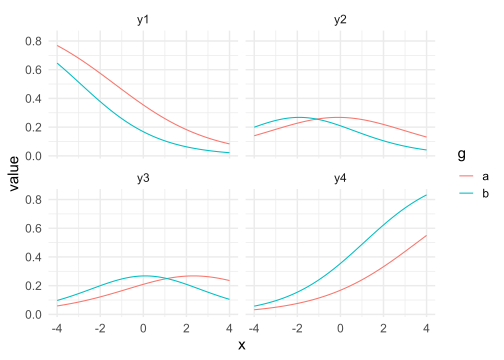
\includegraphics{paper-new_files/figure-latex/unnamed-chunk-9-1} 

}

\caption{ }\label{fig:unnamed-chunk-9}
\end{figure}

\normalsize

We can apply the same idea to an ordinal outcome but we need \(k - 1\) equations where \(k\) is the number of ordinal levels. Let's simulate a similar design with a continuous \(x\) predictor and \(k = 4\) options. We fix the baseline probabilities where \(x = 0\) as uniform thus \(p(y_1) = p(y_2) = ... p(y_k) = 1/k\). The general workflow for the simulation is:

\begin{enumerate}
\def\labelenumi{\arabic{enumi}.}
\tightlist
\item
  Define \(n\) (number of observations) and \(k\) (number of ordinal outcomes)
\item
  Define the regression coefficients \(\beta\)s
\item
  Define the baseline probabilities when \(x = 0\). These probabilities can be converted to the corresponding thresholds \(\alpha\) choosing the appropriate link function (\emph{logit} or \emph{probit}).
\item
  Calculate the linear predictors \(\eta\) using \(k - 1\) equations combining the predictors \(\mathbf{X}\) and regression coefficients \(\mathbf{\beta}\).
\item
  Apply the inverse of the link function \(g^{-1}(\eta)\) on the linear predictor and calculate the cumulative probabilities \(p(y \leq 1|x), p(y \leq 2|x), ... p(y \leq k - 1|x)\).
\item
  Calculate for each observation the probability of the \(k\) outcome as the difference between cumulative probabilities. \(p(y = 1) = 0 - p(y <= 1), p(y = 2) = p(y <= 2) - p(y <= 1)\) (sistema qua). This is implemented in R by adding a columns of zeros and ones respectively at the beginning and end of the matrix of cumulative probabilities.
\item
  Sample \(n\) outcomes from a multinomial distribution, choosing between \(k\) alternatives with the calculated probabilities.
\end{enumerate}

(rivedi se fare con for)
This can be easily implemented in R. We are using a \texttt{for} loop to improve the clarity of the workflow but using the \texttt{*apply} family of functions can improve the efficiency of the computations.

\scriptsize

\normalsize

The linear predictors can be seen in the Figure ref. The \(g\) in this case is the cumulative \emph{probit} function \(\Phi\).

\scriptsize

\begin{figure}

{\centering \includegraphics{paper-new_files/figure-latex/unnamed-chunk-11-1} 

}

\caption{ }\label{fig:unnamed-chunk-11}
\end{figure}

\normalsize

Now we can apply the inverse of the link function \(g^{-1} = \Phi^{-1}\) to calculate the corresponding cumulative probabilities.

\scriptsize

\normalsize

\scriptsize

\begin{verbatim}
##    p_y1  p_y2  p_y3  p_y4
## 1 0.529 0.243  0.15 0.077
## 2 0.242 0.248 0.252 0.258
## 3 0.553 0.237 0.141 0.069
## 4 0.166 0.218 0.264 0.352
## 5   ...   ...   ...   ...
## 6  0.22 0.241 0.257 0.282
## 7 0.357 0.264 0.216 0.163
## 8 0.464 0.256 0.175 0.104
## 9 0.173 0.221 0.263 0.342
\end{verbatim}

\normalsize

We can plot the expected effect of \(\beta_1\) on the \(k\) probabilities using the \texttt{num\_latent\_plot()} function (see Figure \ref{fig:sim-with-probs-lat-plot}). Finally we sample using the \texttt{sample()} function using the calculated probabilities.

\scriptsize

\begin{figure}

{\centering \includegraphics{paper-new_files/figure-latex/sim-with-probs-lat-plot-1} 

}

\caption{sim-with-probs-lat-plot}\label{fig:sim-with-probs-lat-plot}
\end{figure}

\normalsize

\scriptsize

\normalsize

To check the simulation result we can increase the number of observations, fit the model using the \texttt{ordinal::clm()} function and assess the recovery of simulated parameters.

\scriptsize

\normalsize

\scriptsize

\normalsize

\subsubsection{simulating using latent distribution}\label{simulating-using-latent-distribution}

An equivalent but more efficient way to simulate an ordinal outcome is using the latent formulation of the model. This require simulating a standard linear regression using the appropriate data generation function (\emph{logistic} or \emph{normal}) and the cutting the latent values according to the thresholds \(\alpha\). The workflow is slighlty different compared to the previous paragraph:

\begin{enumerate}
\def\labelenumi{\arabic{enumi}.}
\tightlist
\item
  Define \(n\) (number of observations) and \(k\) (number of ordinal outcomes)
\item
  Define the regression coefficients \(\beta\)
\item
  Define the baseline probabilities when \(x = 0\). These probabilities can be converted to the corresponding thresholds \(\alpha\) choosing the appropriate link function (\emph{logit} or \emph{probit}).
\item
  Calculate the linear predictors \(\eta\) using \(k - 1\) equations combining the predictors \(\mathbf{X}\), the regression coefficients \(\mathbf{\beta}\) and the error \(\mathbf{\epsilon}\) sampled from the appropriate probability distribution.
\item
  Cut the latent variable into \(k\) areas using the thresholds \(\alpha\) and assign the corresponding ordinal value. This step simply checks if the latent value \(Y^{\star}_i\) is between two threshold values and assign the corresponding value. This can be done using the \texttt{cut()} or the \texttt{findInterval()} functions.
\end{enumerate}

\scriptsize

\normalsize

The Figure (put crossref) depict the simulated \(Y^{*}\) and the corresponding ordinal value. As for the previous simulation we can fit the model using \texttt{clm()} and check the estimated parameters.

\scriptsize

\begin{figure}

{\centering \includegraphics{paper-new_files/figure-latex/unnamed-chunk-17-1} 

}

\caption{ }\label{fig:unnamed-chunk-17}
\end{figure}

\normalsize

\scriptsize

\normalsize

\scriptsize

\normalsize

The simulation using the latent formulation of the model is implemented in the \texttt{sim\_ord\_latent()} function.

\scriptsize

\begin{Shaded}
\begin{Highlighting}[]
\NormalTok{sim\_ord\_latent }\OtherTok{\textless{}{-}} \ControlFlowTok{function}\NormalTok{(location,}
                           \AttributeTok{scale =} \ConstantTok{NULL}\NormalTok{,}
\NormalTok{                           By,}
                           \AttributeTok{Bscale =} \ConstantTok{NULL}\NormalTok{,}
                           \AttributeTok{probs =} \ConstantTok{NULL}\NormalTok{, }
                           \AttributeTok{alphas =} \ConstantTok{NULL}\NormalTok{, }
\NormalTok{                           data, }
                           \AttributeTok{link =} \FunctionTok{c}\NormalTok{(}\StringTok{"logit"}\NormalTok{, }\StringTok{"probit"}\NormalTok{))\{}
  
  \CommentTok{\# get all the correct functions according to the link}
\NormalTok{  lf }\OtherTok{\textless{}{-}} \FunctionTok{get\_link}\NormalTok{(link)}
  \ControlFlowTok{if}\NormalTok{(}\FunctionTok{is.null}\NormalTok{(alphas))\{}
    \CommentTok{\# calculate thresholds if not provided}
\NormalTok{    alphas }\OtherTok{\textless{}{-}} \FunctionTok{prob\_to\_alpha}\NormalTok{(probs, }\AttributeTok{link =}\NormalTok{ link)}
\NormalTok{  \}}
\NormalTok{  k }\OtherTok{\textless{}{-}} \FunctionTok{length}\NormalTok{(alphas) }\SpecialCharTok{+} \DecValTok{1} \CommentTok{\# number of ordinal outcomes}
\NormalTok{  n }\OtherTok{\textless{}{-}} \FunctionTok{nrow}\NormalTok{(data) }\CommentTok{\# number of observations}
  
  \CommentTok{\# model matrix for the location effect}
\NormalTok{  Xy }\OtherTok{\textless{}{-}} \FunctionTok{model.matrix}\NormalTok{(location, }\AttributeTok{data =}\NormalTok{ data)[, }\SpecialCharTok{{-}}\DecValTok{1}\NormalTok{, drop }\OtherTok{=} \ConstantTok{FALSE}\NormalTok{] }\CommentTok{\# remove intercept}
\NormalTok{  lpy }\OtherTok{\textless{}{-}} \FunctionTok{c}\NormalTok{(Xy }\SpecialCharTok{\%*\%}\NormalTok{ By) }\CommentTok{\# linear predictor for the location}
\NormalTok{  lps }\OtherTok{\textless{}{-}} \DecValTok{0} \CommentTok{\# default scale effect 0, exp(0) = 1 (the default scale)}
  
  \CommentTok{\# check predictors on the scale parameter}
  \ControlFlowTok{if}\NormalTok{(}\SpecialCharTok{!}\FunctionTok{is.null}\NormalTok{(scale))\{}
    \CommentTok{\# model matrix for the scale effect}
\NormalTok{    Xsigma }\OtherTok{\textless{}{-}} \FunctionTok{model.matrix}\NormalTok{(scale, }\AttributeTok{data =}\NormalTok{ data)[, }\SpecialCharTok{{-}}\DecValTok{1}\NormalTok{, drop }\OtherTok{=} \ConstantTok{FALSE}\NormalTok{] }\CommentTok{\# remove intercept}
\NormalTok{    lps }\OtherTok{\textless{}{-}} \FunctionTok{c}\NormalTok{(Xsigma }\SpecialCharTok{\%*\%}\NormalTok{ Bscale) }\CommentTok{\# linear predictor for the scale}
\NormalTok{  \}}
  
  \CommentTok{\# latent variable with appropriate error function}
\NormalTok{  ystar }\OtherTok{\textless{}{-}}\NormalTok{ lf}\SpecialCharTok{$}\FunctionTok{rfun}\NormalTok{(n, lpy, }\FunctionTok{exp}\NormalTok{(lps))}
  
  \CommentTok{\# cut according to thresholds}
\NormalTok{  y }\OtherTok{\textless{}{-}} \FunctionTok{findInterval}\NormalTok{(ystar, alphas) }\SpecialCharTok{+} \DecValTok{1} \CommentTok{\# to start from 1}
  
\NormalTok{  data}\SpecialCharTok{$}\NormalTok{y }\OtherTok{\textless{}{-}} \FunctionTok{ordered}\NormalTok{(y) }\CommentTok{\# to ordered factor}
\NormalTok{  data}\SpecialCharTok{$}\NormalTok{ys }\OtherTok{\textless{}{-}}\NormalTok{ ystar }\CommentTok{\# save also the latent}
  \FunctionTok{return}\NormalTok{(data)}
\NormalTok{\}}
\end{Highlighting}
\end{Shaded}

\normalsize

\subsection{Scale Effects}\label{scale-effects}

The default ordinal regression model assume that the variance of th underlying latent distribution is the same across condition. This is similar to a standard linear regression assuming homogeneity of variance. For example, when comparing two groups or conditions we can run a standard linear model (i.e., a t-test) assuming homogeneity of variances or using the Welch t-test (see Delacre, Lakens, \& Leys, 2017). In addition, there are the so-called location-scale models that allows to include predictors also for the scale (e.g., the variance) of the distribution. This can be done also in ordinal regression where instead of assuming the same variance between conditions, the linear predictors can be included. Figure \ref{fig:example-unequal-variance} depict an example of a comparison between two groups where the two underlyning latent distributions have unequal variance.

spiegare qui che i location-scale models sono sostanzialmente un cambiamento delle soglie (e non dei beta) in funzione di predittori Gerhard Tutz and Berger (2020)

dire che gli scale effects possono essere visti come un'alterativa più parsimoniosa a modelli non-proportional odds Christensen (2019)

se citi brms per modelli più complicati, ricordati di specificare che:

\begin{quote}
That is, s = 1/disc. Further, because disc must be strictly positive, it is by default modeled on the log scale.
\end{quote}

un modo intuitivo per spiegare gli scale effects è di far capire la relazione tra slope e scale. La slope della funzione cumulative corrisponde alla varianza. Se la slope è piuù steep, la varianza sarà minore e la discrimizione maggiore (in \texttt{brms} si chiama desc)

\scriptsize

\normalsize

si può citare anche questo Cox (1995) come riferimento per i modelli

una distinzione tra location-shift and location-scale models G. Tutz and Berger (2017) dove i primi oltre ad un cambiamento di location prevedono un cambiamento di soglie mentre i secondi modellano la differenza di soglie come un cambiamento della scala (varianza) che quindi permette di aumetare o diminuire l'area associata ad un determinato intervallo.

sempre in G. Tutz and Berger (2017) propongono il location-scale/shift come una via di mezzo tra il proportional odds ed il non proportional odds

\subsubsection{Simulating scale effects}\label{simulating-scale-effects}

The location-scale model can be simulated using the \texttt{sim\_ord\_latent()} function and providing the predictors for the scale parameters. Given the \texttt{log} link function, predictors are provided on the \texttt{log} scale. For example, we simulate the effect of a binary variable \(x\) representing two independent groups predicting the \(k = 5\) response. We simulate a \emph{location} effect of \(\beta_1 = 0.5\) (in \emph{probit} scale) and \(\zeta_1 = \text{log}(2) = 0.70\). The first group has a \(\sigma = 1\) and the second group has \(\sigma = 2\). Again we simulate that the baseline probabilities are uniform for the first group.

\scriptsize

\normalsize

The table (put ref) reports the simulation results.

\scriptsize

\normalsize

\subsection{Visualizing effects}\label{visualizing-effects}

Before starting with the actual simulation it is useful to plot the predicted probabilities of the response variable \(y\) as a function of the predictors. The \texttt{cat\_latent\_plot()} and the \texttt{num\_latent\_plot()} functions are able to visualize the effect of a single categorical or numerical predictor. Specifying the mean and standard deviations of the latent variable in each condition (for the categorical version) or the \(\beta\) (for the numerical version) the function compute the expected probability for each level of the ordinal variable \(y\) and visualize the result. In this way the \(\beta\) can be choose in a meaningful way.

\scriptsize

\begin{Shaded}
\begin{Highlighting}[]
\NormalTok{cat\_latent\_plot }\OtherTok{\textless{}{-}} \ControlFlowTok{function}\NormalTok{(}\AttributeTok{m =} \DecValTok{0}\NormalTok{, }
                            \AttributeTok{s =} \DecValTok{1}\NormalTok{, }
                            \AttributeTok{th =} \ConstantTok{NULL}\NormalTok{, }
                            \AttributeTok{probs =} \ConstantTok{NULL}\NormalTok{, }
                            \AttributeTok{link =} \FunctionTok{c}\NormalTok{(}\StringTok{"logit"}\NormalTok{, }\StringTok{"probit"}\NormalTok{),}
                            \AttributeTok{plot =} \FunctionTok{c}\NormalTok{(}\StringTok{"probs"}\NormalTok{, }\StringTok{"latent"}\NormalTok{, }\StringTok{"both"}\NormalTok{))\{}
  \FunctionTok{require}\NormalTok{(ggplot2)}
\NormalTok{  plot }\OtherTok{\textless{}{-}} \FunctionTok{match.arg}\NormalTok{(plot)}
\NormalTok{  lf }\OtherTok{\textless{}{-}} \FunctionTok{get\_link}\NormalTok{(link)}
\NormalTok{  x }\OtherTok{\textless{}{-}} \FunctionTok{paste0}\NormalTok{(}\StringTok{"g"}\NormalTok{, }\DecValTok{1}\SpecialCharTok{:}\FunctionTok{length}\NormalTok{(m))}
\NormalTok{  lat }\OtherTok{\textless{}{-}} \FunctionTok{data.frame}\NormalTok{(}
    \AttributeTok{x =}\NormalTok{ x,}
    \AttributeTok{m =}\NormalTok{ m,}
    \AttributeTok{s =}\NormalTok{ s}
\NormalTok{  )}
  
  \ControlFlowTok{if}\NormalTok{(}\FunctionTok{is.null}\NormalTok{(th))\{}
\NormalTok{    th }\OtherTok{\textless{}{-}} \FunctionTok{prob\_to\_alpha}\NormalTok{(probs, link)}
\NormalTok{  \}}
  
\NormalTok{  thl }\OtherTok{\textless{}{-}}\NormalTok{ latex2exp}\SpecialCharTok{::}\FunctionTok{TeX}\NormalTok{(}\FunctionTok{sprintf}\NormalTok{(}\StringTok{"$}\SpecialCharTok{\textbackslash{}\textbackslash{}}\StringTok{alpha\_\{\%s\}$"}\NormalTok{, }\DecValTok{1}\SpecialCharTok{:}\FunctionTok{length}\NormalTok{(th)))}
  
  \ControlFlowTok{if}\NormalTok{(link }\SpecialCharTok{==} \StringTok{"logit"}\NormalTok{)\{}
\NormalTok{    dfun }\OtherTok{\textless{}{-}}\NormalTok{ distributional}\SpecialCharTok{::}\NormalTok{dist\_logistic}
\NormalTok{    s }\OtherTok{\textless{}{-}} \FunctionTok{sqrt}\NormalTok{(}\FunctionTok{vlogit}\NormalTok{(s))}
\NormalTok{    title }\OtherTok{\textless{}{-}} \StringTok{"Logistic Distribution"}
\NormalTok{  \}}\ControlFlowTok{else}\NormalTok{\{}
\NormalTok{    dfun }\OtherTok{\textless{}{-}}\NormalTok{ distributional}\SpecialCharTok{::}\NormalTok{dist\_normal}
\NormalTok{    s }\OtherTok{\textless{}{-}}\NormalTok{ lat}\SpecialCharTok{$}\NormalTok{s}
\NormalTok{    title }\OtherTok{\textless{}{-}} \StringTok{"Normal Distribution"}
\NormalTok{  \}}
\NormalTok{  lat}\SpecialCharTok{$}\NormalTok{dist }\OtherTok{\textless{}{-}} \FunctionTok{dfun}\NormalTok{(lat}\SpecialCharTok{$}\NormalTok{m, lat}\SpecialCharTok{$}\NormalTok{s)}
\NormalTok{  range\_y }\OtherTok{\textless{}{-}} \FunctionTok{c}\NormalTok{(}\FunctionTok{min}\NormalTok{(lat}\SpecialCharTok{$}\NormalTok{m) }\SpecialCharTok{{-}} \FunctionTok{max}\NormalTok{(s) }\SpecialCharTok{*} \DecValTok{5}\NormalTok{, }\FunctionTok{max}\NormalTok{(lat}\SpecialCharTok{$}\NormalTok{m) }\SpecialCharTok{+} \FunctionTok{max}\NormalTok{(s) }\SpecialCharTok{*} \DecValTok{5}\NormalTok{)}

\NormalTok{  lat\_plot }\OtherTok{\textless{}{-}} \FunctionTok{ggplot}\NormalTok{(lat,}
         \FunctionTok{aes}\NormalTok{(}\AttributeTok{x =} \FunctionTok{factor}\NormalTok{(x), }\AttributeTok{y =}\NormalTok{ m, }\AttributeTok{dist =}\NormalTok{ dist)) }\SpecialCharTok{+}
\NormalTok{    ggdist}\SpecialCharTok{::}\FunctionTok{stat\_halfeye}\NormalTok{(}\FunctionTok{aes}\NormalTok{(}\AttributeTok{fill =} \FunctionTok{after\_stat}\NormalTok{(}\FunctionTok{factor}\NormalTok{(}\FunctionTok{findInterval}\NormalTok{(y, th) }\SpecialCharTok{+} \DecValTok{1}\NormalTok{))),}
                 \AttributeTok{alpha =} \FloatTok{0.85}\NormalTok{) }\SpecialCharTok{+}
    \FunctionTok{ylim}\NormalTok{(range\_y) }\SpecialCharTok{+}
    \FunctionTok{geom\_hline}\NormalTok{(}\AttributeTok{yintercept =}\NormalTok{ th, }\AttributeTok{linetype =} \StringTok{"dashed"}\NormalTok{, }\AttributeTok{col =} \StringTok{"black"}\NormalTok{, }\AttributeTok{alpha =} \FloatTok{0.7}\NormalTok{) }\SpecialCharTok{+}
    \FunctionTok{geom\_line}\NormalTok{(}\FunctionTok{aes}\NormalTok{(}\AttributeTok{x =} \FunctionTok{factor}\NormalTok{(x), }\AttributeTok{y =}\NormalTok{ m, }\AttributeTok{group =} \DecValTok{1}\NormalTok{)) }\SpecialCharTok{+}
    \FunctionTok{annotate}\NormalTok{(}\StringTok{"label"}\NormalTok{, }\AttributeTok{x =} \FloatTok{0.7}\NormalTok{, }\AttributeTok{y =}\NormalTok{ th, }\AttributeTok{label =}\NormalTok{ thl, }\AttributeTok{size =} \DecValTok{5}\NormalTok{) }\SpecialCharTok{+}
    \FunctionTok{theme\_minimal}\NormalTok{(}\DecValTok{15}\NormalTok{) }\SpecialCharTok{+}
    \FunctionTok{theme}\NormalTok{(}\AttributeTok{legend.position =} \StringTok{"bottom"}\NormalTok{,}
          \AttributeTok{legend.title =} \FunctionTok{element\_blank}\NormalTok{(),}
          \AttributeTok{axis.title.x =} \FunctionTok{element\_blank}\NormalTok{()) }\SpecialCharTok{+}
    \FunctionTok{ylab}\NormalTok{(latex2exp}\SpecialCharTok{::}\FunctionTok{TeX}\NormalTok{(}\StringTok{"}\SpecialCharTok{\textbackslash{}\textbackslash{}}\StringTok{mu"}\NormalTok{)) }\SpecialCharTok{+}
    \FunctionTok{ggtitle}\NormalTok{(title)}
  
  
\NormalTok{  th }\OtherTok{\textless{}{-}} \FunctionTok{c}\NormalTok{(}\SpecialCharTok{{-}}\ConstantTok{Inf}\NormalTok{, th, }\ConstantTok{Inf}\NormalTok{)}
\NormalTok{  lat\_ms }\OtherTok{\textless{}{-}}\NormalTok{ lat[, }\FunctionTok{c}\NormalTok{(}\StringTok{"m"}\NormalTok{, }\StringTok{"s"}\NormalTok{)]}
\NormalTok{  ps }\OtherTok{\textless{}{-}} \FunctionTok{apply}\NormalTok{(lat\_ms, }\DecValTok{1}\NormalTok{, }\ControlFlowTok{function}\NormalTok{(x) }\FunctionTok{data.frame}\NormalTok{(}\FunctionTok{t}\NormalTok{(}\FunctionTok{diff}\NormalTok{(lf}\SpecialCharTok{$}\FunctionTok{pfun}\NormalTok{(th, x[}\DecValTok{1}\NormalTok{], x[}\DecValTok{2}\NormalTok{])))), }\AttributeTok{simplify =} \ConstantTok{FALSE}\NormalTok{)}
\NormalTok{  ps }\OtherTok{\textless{}{-}} \FunctionTok{do.call}\NormalTok{(rbind, ps)}
  \FunctionTok{names}\NormalTok{(ps) }\OtherTok{\textless{}{-}} \FunctionTok{paste0}\NormalTok{(}\StringTok{"y"}\NormalTok{, }\DecValTok{1}\SpecialCharTok{:}\FunctionTok{ncol}\NormalTok{(ps))}
\NormalTok{  latl }\OtherTok{\textless{}{-}} \FunctionTok{cbind}\NormalTok{(lat, ps)}
\NormalTok{  latl }\OtherTok{\textless{}{-}}\NormalTok{ tidyr}\SpecialCharTok{::}\FunctionTok{pivot\_longer}\NormalTok{(latl, }\FunctionTok{starts\_with}\NormalTok{(}\StringTok{"y"}\NormalTok{), }\AttributeTok{names\_to =} \StringTok{"y"}\NormalTok{, }\AttributeTok{values\_to =} \StringTok{"value"}\NormalTok{)}
\NormalTok{  probs\_plot }\OtherTok{\textless{}{-}} \FunctionTok{ggplot}\NormalTok{(latl, }\FunctionTok{aes}\NormalTok{(}\AttributeTok{x =} \FunctionTok{factor}\NormalTok{(x), }\AttributeTok{y =}\NormalTok{ value, }\AttributeTok{fill =}\NormalTok{ y)) }\SpecialCharTok{+}
    \FunctionTok{geom\_col}\NormalTok{(}\AttributeTok{position =} \FunctionTok{position\_dodge}\NormalTok{()) }\SpecialCharTok{+}
    \FunctionTok{theme\_minimal}\NormalTok{(}\DecValTok{15}\NormalTok{) }\SpecialCharTok{+}
    \FunctionTok{theme}\NormalTok{(}\AttributeTok{legend.position =} \StringTok{"bottom"}\NormalTok{,}
          \AttributeTok{legend.title =} \FunctionTok{element\_blank}\NormalTok{(),}
          \AttributeTok{axis.title.x =} \FunctionTok{element\_blank}\NormalTok{()) }\SpecialCharTok{+}
    \FunctionTok{ylab}\NormalTok{(}\StringTok{"Probability"}\NormalTok{)}
  \ControlFlowTok{if}\NormalTok{(plot }\SpecialCharTok{==} \StringTok{"probs"}\NormalTok{)\{}
\NormalTok{    probs\_plot}
\NormalTok{  \}}\ControlFlowTok{else} \ControlFlowTok{if}\NormalTok{(plot }\SpecialCharTok{==} \StringTok{"latent"}\NormalTok{)\{}
\NormalTok{    lat\_plot}
\NormalTok{  \}}\ControlFlowTok{else}\NormalTok{\{}
\NormalTok{    legend\_b }\OtherTok{\textless{}{-}}\NormalTok{ cowplot}\SpecialCharTok{::}\FunctionTok{get\_legend}\NormalTok{(}
\NormalTok{      probs\_plot}
\NormalTok{    )}
\NormalTok{    plts }\OtherTok{\textless{}{-}}\NormalTok{ cowplot}\SpecialCharTok{::}\FunctionTok{plot\_grid}\NormalTok{(}
\NormalTok{      lat\_plot }\SpecialCharTok{+} \FunctionTok{theme}\NormalTok{(}\AttributeTok{legend.position =} \StringTok{"none"}\NormalTok{),}
\NormalTok{      probs\_plot }\SpecialCharTok{+} \FunctionTok{theme}\NormalTok{(}\AttributeTok{legend.position =} \StringTok{"none"}\NormalTok{)}
\NormalTok{    )}
\NormalTok{    cowplot}\SpecialCharTok{::}\FunctionTok{plot\_grid}\NormalTok{(plts, legend\_b, }\AttributeTok{ncol =} \DecValTok{1}\NormalTok{, }\AttributeTok{rel\_heights =} \FunctionTok{c}\NormalTok{(}\DecValTok{1}\NormalTok{, .}\DecValTok{1}\NormalTok{))}
\NormalTok{  \}}
\NormalTok{\}}
\NormalTok{num\_latent\_plot }\OtherTok{\textless{}{-}} \ControlFlowTok{function}\NormalTok{(x, }
\NormalTok{                            b1, }
                            \AttributeTok{th =} \ConstantTok{NULL}\NormalTok{, }
                            \AttributeTok{probs =} \ConstantTok{NULL}\NormalTok{,}
                            \AttributeTok{link =} \FunctionTok{c}\NormalTok{(}\StringTok{"logit"}\NormalTok{, }\StringTok{"probit"}\NormalTok{), }
                            \AttributeTok{nsample =} \FloatTok{1e3}\NormalTok{, }
                            \AttributeTok{size =} \DecValTok{20}\NormalTok{)\{}
\NormalTok{  lf }\OtherTok{\textless{}{-}} \FunctionTok{get\_link}\NormalTok{(link)}
  \ControlFlowTok{if}\NormalTok{(}\FunctionTok{is.null}\NormalTok{(th))\{}
\NormalTok{    th }\OtherTok{\textless{}{-}} \FunctionTok{prob\_to\_alpha}\NormalTok{(probs, link)}
\NormalTok{  \}}
\NormalTok{  data }\OtherTok{\textless{}{-}} \FunctionTok{data.frame}\NormalTok{(}\AttributeTok{x =} \FunctionTok{seq}\NormalTok{(}\FunctionTok{min}\NormalTok{(x), }\FunctionTok{max}\NormalTok{(x), }\AttributeTok{length.out =}\NormalTok{ nsample))}
\NormalTok{  data }\OtherTok{\textless{}{-}} \FunctionTok{get\_probs}\NormalTok{(}\SpecialCharTok{\textasciitilde{}}\NormalTok{x, b1, probs, data, link, }\AttributeTok{append =} \ConstantTok{TRUE}\NormalTok{)}
\NormalTok{  datal }\OtherTok{\textless{}{-}}\NormalTok{ tidyr}\SpecialCharTok{::}\FunctionTok{pivot\_longer}\NormalTok{(data, }\FunctionTok{starts\_with}\NormalTok{(}\StringTok{"y"}\NormalTok{), }\AttributeTok{names\_to =} \StringTok{"y"}\NormalTok{, }\AttributeTok{values\_to =} \StringTok{"value"}\NormalTok{)}
  \FunctionTok{ggplot}\NormalTok{(datal, }\FunctionTok{aes}\NormalTok{(}\AttributeTok{x =}\NormalTok{ x, }\AttributeTok{y =}\NormalTok{ value, }\AttributeTok{color =}\NormalTok{ y)) }\SpecialCharTok{+}
    \FunctionTok{geom\_line}\NormalTok{() }\SpecialCharTok{+}
    \FunctionTok{theme\_minimal}\NormalTok{(size) }\SpecialCharTok{+}
    \FunctionTok{theme}\NormalTok{(}\AttributeTok{legend.position =} \StringTok{"bottom"}\NormalTok{,}
          \AttributeTok{legend.title =} \FunctionTok{element\_blank}\NormalTok{()) }\SpecialCharTok{+}
    \FunctionTok{ylab}\NormalTok{(}\StringTok{"Probability"}\NormalTok{) }\SpecialCharTok{+}
    \FunctionTok{ggtitle}\NormalTok{(latex2exp}\SpecialCharTok{::}\FunctionTok{TeX}\NormalTok{(}\FunctionTok{sprintf}\NormalTok{(}\StringTok{"$}\SpecialCharTok{\textbackslash{}\textbackslash{}}\StringTok{beta\_1 = \%s$"}\NormalTok{, b1)))}
\NormalTok{\}}
\end{Highlighting}
\end{Shaded}

\normalsize

For example, the Figure \ref{fig:ex-categorical} depicts the effect of a categorical predictor on a 5-level \(y\) assuming uniform probabilities for the reference level and a mean difference on a standardized Normal distribution of 1. The Figure \ref{fig:ex-numerical} depicts the effect of a continuous predictor \(x\) sampled from a standard Normal distribution assuming a \(\beta = 1\).

\scriptsize

\begin{figure}

{\centering \includegraphics{paper-new_files/figure-latex/ex-categorical-1} 

}

\caption{Example categorical}\label{fig:ex-categorical}
\end{figure}

\normalsize

\scriptsize

\begin{figure}

{\centering \includegraphics{paper-new_files/figure-latex/ex-numerical-1} 

}

\caption{Example numerical}\label{fig:ex-numerical}
\end{figure}

\normalsize

\subsection{Disclaimer about the functions}\label{disclaimer-about-the-functions}

The current paper proposed a simplified way with some functions to generate ordinal data. For more complex simulations such as simulating correlated ordinal data the \texttt{simstudy} package \url{https://kgoldfeld.github.io/simstudy/articles/ordinal.html} proposed a very comprehensive set of data simulation function also for ordinal data.

\newpage

\section{References}\label{references}

\phantomsection\label{refs}
\begin{CSLReferences}{1}{0}
\bibitem[\citeproctext]{ref-Burkner2019-aw}
Bürkner, P.-C., \& Vuorre, M. (2019). Ordinal regression models in psychology: A tutorial. \emph{Advances in Methods and Practices in Psychological Science}, \emph{2}, 77--101. \url{https://doi.org/10.1177/2515245918823199}

\bibitem[\citeproctext]{ref-Christensen2019-cz}
Christensen, R. H. B. (2019). \emph{Ordinal---regression models for ordinal data}.

\bibitem[\citeproctext]{ref-Cliff2016-ck}
Cliff, N. (2016). \emph{Ordinal methods for behavioral data analysis}. London, England: Psychology Press.

\bibitem[\citeproctext]{ref-Cox1995-ur}
Cox, C. (1995). Location-scale cumulative odds models for ordinal data: A generalized non-linear model approach. \emph{Statistics in Medicine}, \emph{14}, 1191--1203. \url{https://doi.org/10.1002/sim.4780141105}

\bibitem[\citeproctext]{ref-DeCarlo1998-ay}
DeCarlo, L. T. (1998). Signal detection theory and generalized linear models. \emph{Psychological Methods}, \emph{3}, 186--205. \url{https://doi.org/10.1037/1082-989X.3.2.186}

\bibitem[\citeproctext]{ref-DeCarlo2010-lj}
DeCarlo, L. T. (2010). On the statistical and theoretical basis of signal detection theory and extensions: Unequal variance, random coefficient, and mixture models. \emph{Journal of Mathematical Psychology}, \emph{54}, 304--313. \url{https://doi.org/10.1016/j.jmp.2010.01.001}

\bibitem[\citeproctext]{ref-Delacre2017-qy}
Delacre, M., Lakens, D., \& Leys, C. (2017). Why psychologists should by default use welch's \emph{t}-test instead of student's \emph{t}-test. \emph{International Review of Social Psychology}, \emph{30}, 92. \url{https://doi.org/10.5334/irsp.82}

\bibitem[\citeproctext]{ref-Gelman2020-tg}
Gelman, A., Hill, J., \& Vehtari, A. (2020). \emph{Regression and other stories}. Cambridge University Press. \url{https://doi.org/10.1017/9781139161879}

\bibitem[\citeproctext]{ref-Green1966-gy}
Green, D. M., Swets, J. A., \& Others. (1966). \emph{Signal detection theory and psychophysics} (Vol. 1, pp. xi, 455--xi, 455). Oxford, England: Wiley New York.

\bibitem[\citeproctext]{ref-Harrell-2015-no}
Harrell, F. E. (2015). \emph{Regression modeling strategies}. Cham: Springer International Publishing. \url{https://doi.org/10.1007/978-3-319-19425-7}

\bibitem[\citeproctext]{ref-Kemp2021-dj}
Kemp, S., \& Grace, R. C. (2021). Using ordinal scales in psychology. \emph{Methods in Psychology (Online)}, \emph{5}, 100054. \url{https://doi.org/10.1016/j.metip.2021.100054}

\bibitem[\citeproctext]{ref-Knoblauch2012-to}
Knoblauch, K., \& Maloney, L. T. (2012). \emph{Modeling psychophysical data in r}. New York, NY: Springer New York. \url{https://doi.org/10.1007/978-1-4614-4475-6}

\bibitem[\citeproctext]{ref-Kruschke2015-re}
Kruschke, J. K. (2015). \emph{Doing bayesian data analysis}. \url{https://doi.org/10.1016/c2012-0-00477-2}

\bibitem[\citeproctext]{ref-Kurz2023-zv}
Kurz, A. S. (2023). \emph{Doing bayesian data analysis in brms and the tidyverse} (Version 1.1.0). Retrieved from \url{https://bookdown.org/content/3686/}

\bibitem[\citeproctext]{ref-Liddell2018-wu}
Liddell, T. M., \& Kruschke, J. K. (2018). Analyzing ordinal data with metric models: What could possibly go wrong? \emph{Journal of Experimental Social Psychology}, \emph{79}, 328--348. \url{https://doi.org/10.1016/j.jesp.2018.08.009}

\bibitem[\citeproctext]{ref-Likert1932-xw}
Likert, R. (1932). A technique for the measurement of attitudes. \emph{Archives of Psychology}, \emph{22}, 55. Retrieved from \url{https://psycnet.apa.org/record/1933-01885-001}

\bibitem[\citeproctext]{ref-Liu2023-bp}
Liu, A., He, H., Tu, X. M., \& Tang, W. (2023). On testing proportional odds assumptions for proportional odds models. \emph{General Psychiatry}, \emph{36}, e101048. \url{https://doi.org/10.1136/gpsych-2023-101048}

\bibitem[\citeproctext]{ref-McCullagh1980-cw}
McCullagh, P. (1980). Regression models for ordinal data. \emph{Journal of the Royal Statistical Society}, \emph{42}, 109--127. \url{https://doi.org/10.1111/j.2517-6161.1980.tb01109.x}

\bibitem[\citeproctext]{ref-Rigby2005-ko}
Rigby, R. A., \& Stasinopoulos, D. M. (2005). Generalized additive models for location, scale and shape. \emph{Journal of the Royal Statistical Society. Series C, Applied Statistics}, \emph{54}, 507--554. \url{https://doi.org/10.1111/j.1467-9876.2005.00510.x}

\bibitem[\citeproctext]{ref-Robitzsch2020-la}
Robitzsch, A. (2020). Why ordinal variables can (almost) always be treated as continuous variables: Clarifying assumptions of robust continuous and ordinal factor analysis estimation methods. \emph{Frontiers in Education}, \emph{5}, 589965. \url{https://doi.org/10.3389/feduc.2020.589965}

\bibitem[\citeproctext]{ref-Stanislaw1999-jr}
Stanislaw, H., \& Todorov, N. (1999). Calculation of signal detection theory measures. \emph{Behavior Research Methods, Instruments, \& Computers: A Journal of the Psychonomic Society, Inc}, \emph{31}, 137--149. \url{https://doi.org/10.3758/bf03207704}

\bibitem[\citeproctext]{ref-Stevens1946-te}
Stevens, S. S. (1946). On the theory of scales of measurement. \emph{Science (New York, N.Y.)}, \emph{103}, 677--680. \url{https://doi.org/10.1126/science.103.2684.677}

\bibitem[\citeproctext]{ref-Tutz1990-fe}
Tutz, Gerhard. (1990). Sequential item response models with an ordered response. \emph{The British Journal of Mathematical and Statistical Psychology}, \emph{43}, 39--55. \url{https://doi.org/10.1111/j.2044-8317.1990.tb00925.x}

\bibitem[\citeproctext]{ref-Tutz2022-dg}
Tutz, Gerhard. (2022). Ordinal regression: A review and a taxonomy of models. \emph{Wiley Interdisciplinary Reviews. Computational Statistics}, \emph{14}. \url{https://doi.org/10.1002/wics.1545}

\bibitem[\citeproctext]{ref-Tutz2017-de}
Tutz, G., \& Berger, M. (2017). Separating location and dispersion in ordinal regression models. \emph{Econometrics and Statistics}, \emph{2}, 131--148. \url{https://doi.org/10.1016/j.ecosta.2016.10.002}

\bibitem[\citeproctext]{ref-Tutz2020-xq}
Tutz, Gerhard, \& Berger, M. (2020). Non proportional odds models are widely dispensable -- sparser modeling based on parametric and additive location-shift approaches. Retrieved from \url{http://arxiv.org/abs/2006.03914}

\end{CSLReferences}






\end{document}
